\section{Setting up PySimLib}

The following will show you how to set up PySimLib, while mainly focusing on Windows platforms.
Installation instructions for systems based on Ubuntu are also given.
Due to the variety of Linux systems we can't provide installation instructions for all of them.
Unfortunately we currently have no access to a Mac computer and can therefore not provide installation instructions, nor do we know if PySimLib works on Mac at all.
We would be pleased to hear feedback on that.

At first we will give a brief introduction on how to open a command line terminal or console, which will be necessary for the setup process described here.
The first installation step then will be to install Python, as PySimLib is a Python library.
In order to simulate models using the PySimLib you will need a simulator that can simulate your models.
Note that PySimLib is not a simulator itself but can communicate with several ones and provides a common interface to do so.
The second step of installation will be to install a simulator.
After these preparations PySimLib can be installed and finally we will describe how to configure PySimLib correctly.




\subsection{Command line}

The command line terminal or console is a program by which the user can issue commands in text-form.
Interaction is realized in the following way:
The program writes text to the screen that the user can read.
The user writes text commands that are confirmed by the \grqq{}Enter\grqq{} or \grqq{}Return\grqq{} keys and are read and executed by the program.

Usually operating systems come with a command line program, in order to control settings, files etc.
Specific commands may not be executed by any user but by a system administrator, who is allowed to run commands with advanced privileges, such as installing a program or making any other change to the system.

\subsubsection{Windows}
In Microsoft Windows, the utility cmd.exe is included, also called.
In order to open it, click the \grqq{}Start\grqq{}-Button or the Windows-Button.
In the search widget, type \grqq{}cmd\grqq{} without the quotation marks.
The program \grqq{}Command Prompt\grqq{}, \grqq{}cmd.exe\grqq{} or something similar should appear.
Click it in order to start it.
A window similar to that shown in figure \ref{wincmd} should open up.
In order to run the console in adminstrator mode, repeat the above process but instead of doing a left click, click right and press \grqq{}Run as adminstrator\grqq{}.

\begin{figure}[h]
	\centering
	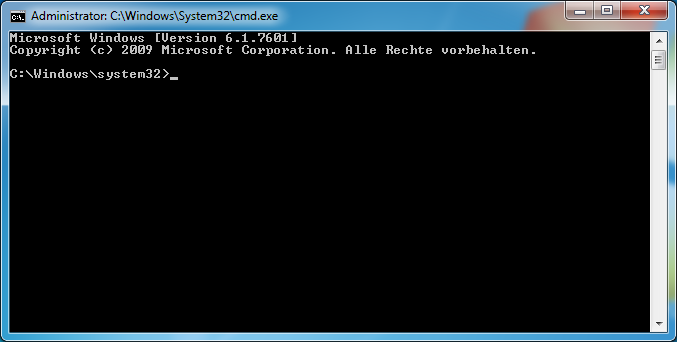
\includegraphics[width=0.5\textwidth]{images/cmd.png}
	\caption{Windows command prompt under Windows 7 in Administrator mode}
	\label{wincmd}
\end{figure}



\subsection{Unix-like}
Usually a command line program, usually called Terminal in Unix world, is included with the operating system.
You should look for it in your program launcher possibly in a category \grqq{}System tools\grqq{} or something close.

You can run a command with advanced privileges by entering the \grqq{}sudo\grqq{} command before it.
Say you want to run the command \grqq{}help\grqq{} with advanced privileges enter \grqq{}sudo help\grqq{} without quotation marks.
This might ask you for the password of your operating systems' user account.





\subsection{Installing Python}

The first step in setting up PySimLib is installing Python.
PySimLib was developed for Python 3, in particular version 3.5.
The library might also work with previous versions of Python 3 but surely not with Python 2.
By us, PySimLib has only been tested in Python 3.5 and we would recommend you to use it.
In general it is more likely that we will support a newer version than an older one than Python 3.5.

In this guide we will expect users to install apart from Python also \grqq{}pip\grqq{} (this will be shown later).
Pip is Pythons' package management utility and allows to easily install extensions to Python.
This is not required, as extensions can be also installed manually but this is rather cumbersome and we don't encourage it.
In case you don't want to use pip, you can download the mentioned packages and install them manually.
We will not give support on this process.


\subsubsection{Windows}

Go to Pythons' website, download the installer and run it.
You should see something like in figure \ref{pythonSetup1}.
You don't need to customize the installation, however we encourage you to check the \grqq{}Add Python 3.5 to PATH\grqq{} box.
This allows you to execute Python from any directory, which is not necessarily required but makes working with Python easier.
Don't select this in case you have other versions of Python installed and one of them is added to the PATH environment variable.
However, in this guide we will expect that the user added Python 3.5 to the PATH variable.
If you did not do that you have to specify the full path to Python whenever you want to use it.

\begin{figure}[h]
	\centering
	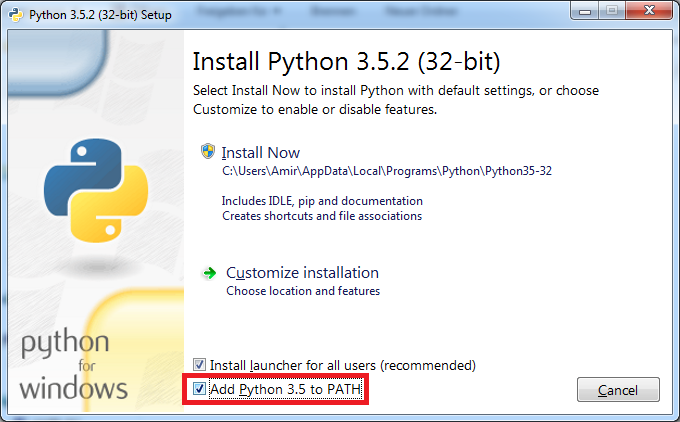
\includegraphics[width=0.5\textwidth]{images/python_setup1.png}
	\caption{Python 3.5 Windows setup}
	\label{pythonSetup1}
\end{figure}


In case you want to customize the installation, make sure, like in figure \ref{pythonSetup2}, that you select at least \grqq{}pip\grqq{} and \grqq{}tcl/tk and IDLE\grqq{}, which is required by PySimLib in order to draw and show plots.

\begin{figure}[H]
	\centering
	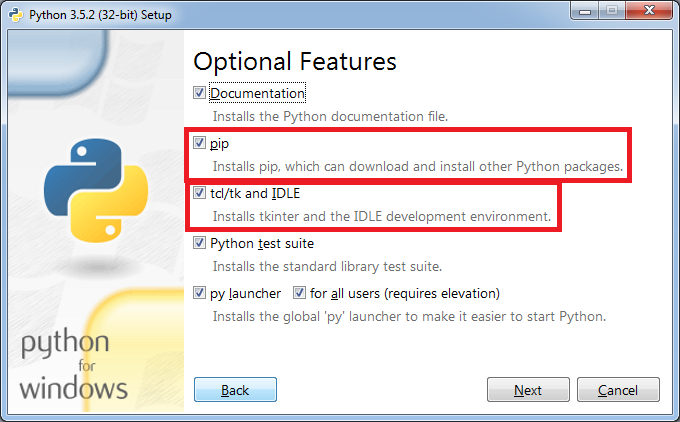
\includegraphics[width=0.5\textwidth]{images/python_setup2.png}
	\caption{Python 3.5 Windows customized setup}
	\label{pythonSetup2}
\end{figure}




\subsubsection{Ubuntu}
Python should already be installed on Ubuntu.
If not, install it by running the following commands:
\lstset{language=bash}
\begin{lstlisting}
sudo apt-get install python3
sudo apt-get install python3-pip
sudo apt-get install python3-tk
\end{lstlisting}
If you are unsure whether Python is installed or not, run the commands anyways.
In case Python is already installed, apt-get is going to inform you and nothing is going to be done.





\subsection{Installing a Simulator}

PySimLib currently supports the simulators listed in table \ref{simulatorsList}.

\begin{table}[h]
	\centering
	\begin{tabular}{| l |}
		\hline
		Dymola \\ \hline
		OpenModelica \\ \hline
		MATLAB/Simulink \\ \hline
	\end{tabular}
	\caption{List of simulators supported by PySimLib}
	\label{simulatorsList}
\end{table}

Please follow the manual of the simulator of your choice in order to set it up correctly.
Be sure that it is working properly before continuing with installing PySimLib.

It should be noted that these simulators exist in different versions, which differentiate in terms of features etc.
We have listed the constellations of operating system and simulator version under which we tested PySimLib in table \ref{testTable}.

\begin{table}[H]
	\centering
	\begin{tabular}{c | c | c | c | c |}
		%header
		&
		\rotatebox{90}{Windows 7 64 bit} &
		\rotatebox{90}{Windows 10 64 bit} &
		\rotatebox{90}{Ubuntu 14.10} &
		\rotatebox{90}{Ubuntu 16.04}
		\\ \hline
		
		%							Win7 x64   & Win10 x64  & Ubuntu 14.10	& Ubuntu 16.04
		Dymola 2013 			&	\checkmark &			& 				& 				\\ \hline
		OpenModelica 1.9.6 		&	           & 			& \checkmark	& \checkmark 	\\ \hline
		MATLAB/Simulink R2013a 	&			   & 			& 				& \checkmark 	\\ \hline
		
	\end{tabular}
	\caption{Testing Constellations of Operating Systems and Simulators using PySimLib}
	\label{testTable}
\end{table}

\textbf{In case you want to use Dymola under Windows you need to install the package \grqq{}pywin32\grqq{} from \url{https://sourceforge.net/projects/pywin32/}.}
PySimLib can also work with a demo version of Dymola but a lot of features will then be unavailable so make sure you have a fully licensed version.

You can install (or remove) additional simulators any time but whenever you do that, you have to reconfigure PySimLib.
See subsection \ref{configuringPySimLib} for configuring PySimLib.





\subsection{Installing PySimLib}

PySimLib can be installed very simply using pip.
In order to determine the correct pip version try entering the following commands:
\lstset{language=bash}
\begin{lstlisting}
pip3.5
pip3
pip
\end{lstlisting}

Remember the first one that worked and take it for all following commands where "pipxyz" is used.
\\
To install PySimLib execute the following commands (\textbf{you might need advanced privileges}):
\begin{lstlisting}
pipxyz install zmq
pipxyz install numpy
pipxyz install PySimLib
\end{lstlisting}






\subsection{Configuring PySimLib}
\label{configuringPySimLib}

In order to have PySimLib communicating with simulators, it must be told certain info, for example which simulator is installed, where is it installed etc.
This is realized by using a global configuration file.
In order to configure PySimLib a normal text editor is sufficient.
\textbf{Important: Only configure simulators that you have installed on your system!}

The name of the configuration file is \texttt{PySimLib.cfg} (beware of the case on Unix-like systems).
On Windows systems, the configuration file must be stored in the \texttt{\%LOCALAPPDATA\%} directory, for Unix-like systems under \texttt{~/.config}.
\texttt{\%LOCALAPPDATA\%} is an environment variable that expands to a specific folder in your user directory, so is \grqq{}~\grqq{} a short cut to the user directory.
You can use the command line and the \grqq{}echo\grqq{} command in order to expand them to fully qualified paths, like so (similar for Unix-like):
\lstset{language=bash}
\begin{lstlisting}
echo %LOCALAPPDATA%
\end{lstlisting}
Note that these folders might be hidden by the file explorer.

\subsubsection{Windows}
In order to create the configuration file, \textbf{in case you haven't created it already as else this might overwrite your configuration file}, enter in console:
\lstset{language=bash}
\begin{lstlisting}
echo. 2>%LOCALAPPDATA%\PySimLib.cfg
\end{lstlisting}

To edit the configuration file, type in console:
\lstset{language=bash}
\begin{lstlisting}
notepad %LOCALAPPDATA%\PySimLib.cfg
\end{lstlisting}




\subsubsection{Unix-like}
Call your text editor with the configuration file path as argument.
For instance, when using Ubuntus text editor \grqq{}gedit\grqq{}:
\lstset{language=bash}
\begin{lstlisting}
gedit ~/.config
\end{lstlisting}




\subsubsection{Configuration file Syntax}
The configuration file consists of sections and key-value pairs attached to them.
A section is introduced by a text in squared brackets, for instance \texttt{[Dymola]} for the \grqq{}Dymola\grqq{} section.
Following the sections are the key-value pairs, the options of the section.
Both key and value are text and they are separated by an equal-sign.
Only one key-value pair per line is allowed.
\textbf{Be aware that the key-value pairs are in general case-sensitive!}

An example of a configuration file with all values for all simulators is shown in listing \ref{configExample}.
Recap to only configure simulators that are installed and working on your system.
The meaning of the configuration values are for the specific simulators are explained in the following subsections.
In general, when asked for a path, the fully qualified path should be preferred, as did in the example for the Dymola and Simulink tools.
\lstset{language=INI,caption={An example configuration file}, label={configExample}}
\begin{lstlisting}
[Dymola]
PathExe=C:\Program Files (x86)\Dymola 2013 FD01\bin\dymola.exe
StartupDelay=8
PathAlist=C:\Program Files (x86)\Dymola 2013 FD01\bin\alist.exe
SimByExe=true

[OpenModelica]
PathExe=omc

[Simulink]
PathExe=/home/amir/MATLAB/R2013a/bin/matlab
\end{lstlisting}




\subsubsection{Configuration Values for Dymola}
\begin{table}[H]
	\centering
	\begin{tabular}{| l | l | p{10cm} |}
	\hline
		\textbf{Configuration key} & \textbf{Value type} & \textbf{Value explanation} \\ \hline
		
		PathExe & Path & The path to the Dymola executable or a command in order to run it. \\ \hline
		
		StartupDelay & Integer & The duration in seconds that PySimLib should wait for Dymola to start up before trying to communicate with it. This setting is highly dependent on the machine you're running PySimLib on. \\ \hline 
		
		PathAlist & Path & The path to the alist executable or a command in order to run it. This utility is shipped with Dymola. \\ \hline
		
		SimByExe & $\lbrace$true, false$\rbrace$ & This should in general be set to true. Only set this to false if you're running Dymola with a demo license. Apart from the general drawbacks of Dymolas demo mode, not all features from PySimLib work. Use this if you want to test working with PySimLib and Dymola together. For efficient working with PySimLib in conjuction with Dymola, you should have a license such that you can run the \grqq{}dymosim\grqq{} executables, that Dymola generates for models, outside of Dymola. \\ \hline
	\end{tabular}
	\caption{Configuration values for Dymola}
\end{table}




\subsubsection{Configuration Values for OpenModelica}
\begin{table}[h]
	\centering
	\begin{tabular}{| l | l | p{10cm} |}
		\hline
		\textbf{Configuration key} & \textbf{Value type} & \textbf{Value explanation} \\ \hline
		
		PathExe & Path & The path to the OpenModelica compiler executable \grqq{}omc\grqq{} or a command in order to run it. \\ \hline
	\end{tabular}
	\caption{Configuration values for OpenModelica}
\end{table}



\subsubsection{Configuration Values for MATLAB/Simulink}
\begin{table}[h]
	\centering
	\begin{tabular}{| l | l | p{10cm} |}
		\hline
		\textbf{Configuration key} & \textbf{Value type} & \textbf{Value explanation} \\ \hline
		
		PathExe & Path & The path to the MATLAB executable or a command in order to run it. \\ \hline
	\end{tabular}
	\caption{Configuration values for MATLAB/Simulink}
\end{table}


\subsection{Updating PySimLib}
You can use Pip again to update PySimLib to its newest version.
Simply execute the following command to do so:
\lstset{language=bash,caption={}, label={}}
\begin{lstlisting}
pipxyz install --upgrade PySimLib
\end{lstlisting}
You may again need advanced privileges.
